\documentclass[uplatex,dvipdfmx]{jsarticle}

\usepackage[uplatex,deluxe]{otf} % UTF
\usepackage[noalphabet]{pxchfon} % must be after otf package
\usepackage{stix2} %欧文&数式フォント
\usepackage[fleqn,tbtags]{mathtools} % 数式関連 (w/ amsmath)
\usepackage{hira-stix} % ヒラギノフォント&STIX2 フォント代替定義(Warning回避)


\usepackage{ascmac}
\usepackage{url}
\usepackage{float}
\usepackage{moreverb}
\usepackage{lscape}

\begin{document}

\title{自転車姿勢制御モジュールの提案}
\author{25G1065 塩澤匠生}
\date{2025年6月11日}
\maketitle
\section{はじめに}

\subsection{社会的背景}

社会的背景として自転車の単独事故は年5497件発生していて,その割合は年々増加している
というものがある\cite{jikokensuu}.
単独事故の割合は,年々増加しているというものがある.そして,
単独事故の原因の内7割が転倒事故であるというものがある\cite{tandokuWariai}.

\subsection{問題点}

ここで,車の単独事故の原因の内訳と比較してみると車の単独事故の内転倒(横転)事故は1\%
であることから,自転車は乗り物の性質上転倒事故が発生するという問題があると考えることができる.



%一般的な社会的背景を記述したパラグラフを複数配置, パラグラフの終わりは\parを入れる。
%最終パラグラフにはアイデアを記述する.

\subsection{目的}
問題を解決することにより,自転車で転倒事故が発生しない,または発生しにくくすることで
自転車の転倒事故を減少させることを目的とする.


\section{解決策としての提案手法}

自転車の性質上,転倒事故が発生しやすいという問題に対して我々は自転車姿勢制御モジュールというものを
提案する.自転車姿勢制御モジュールの概念図を以下図\ref{fig:moduleGainenn}に示す

\begin{figure}[H]
    \centering
    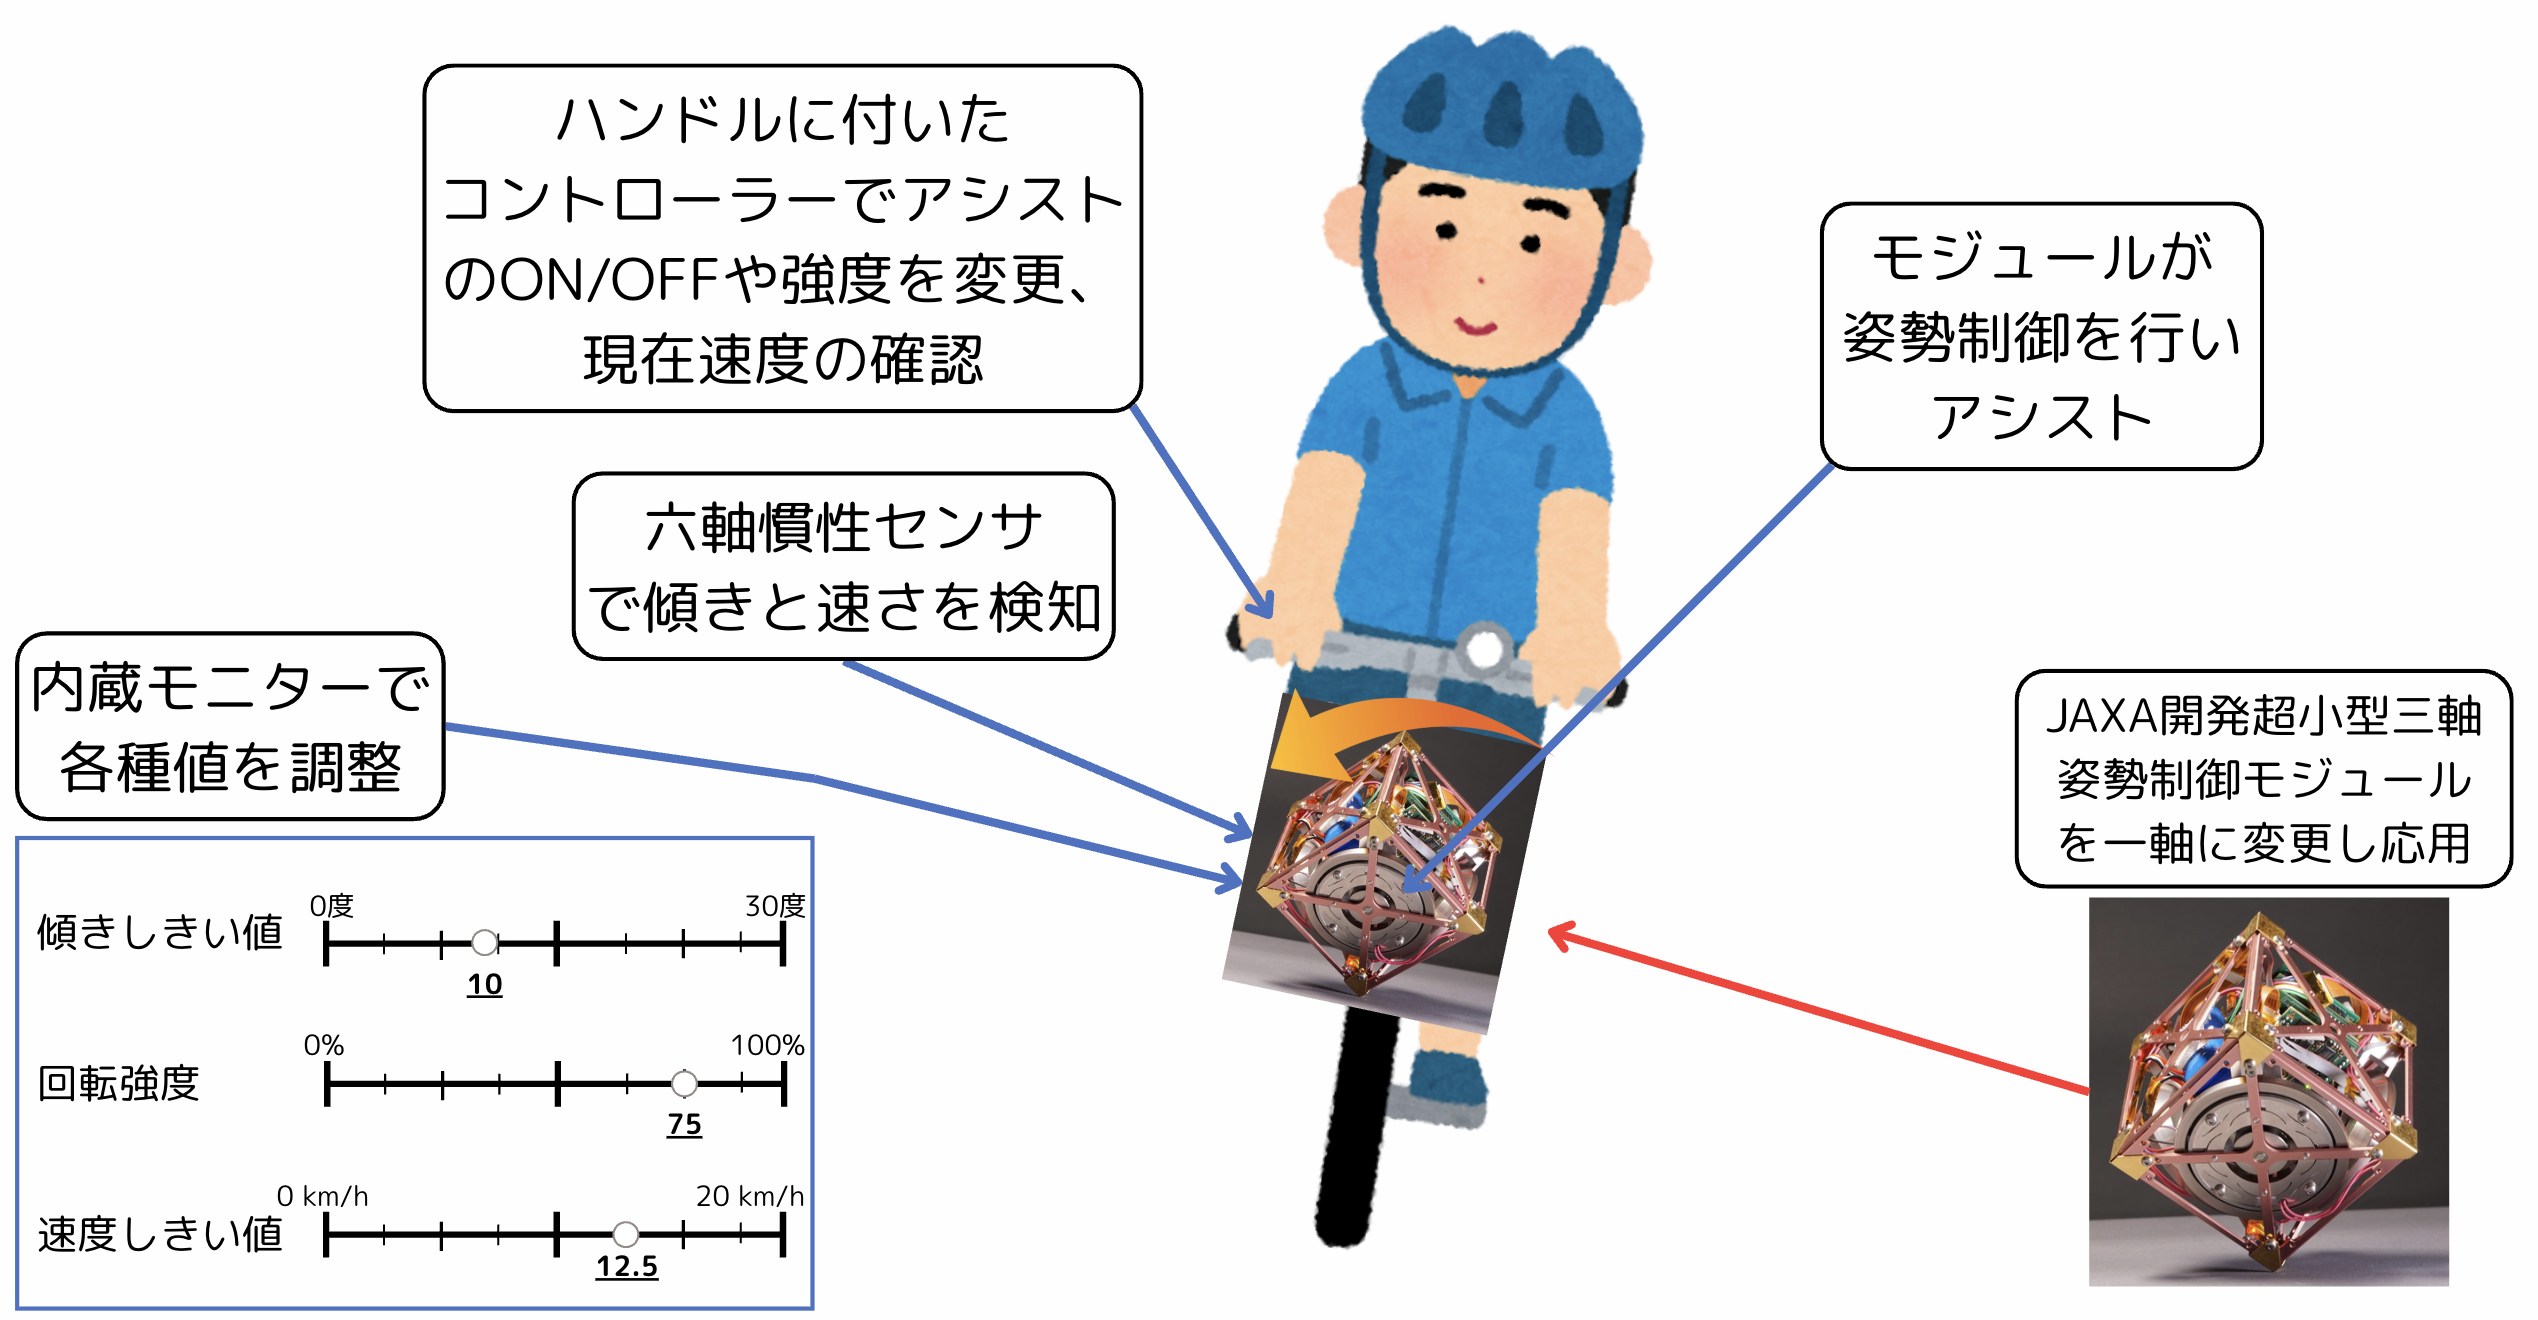
\includegraphics[width=0.8\textwidth]{fig/moduleGainenn2.png}
    \caption{自転車姿勢制御モジュールの概念図}
    \label{fig:moduleGainenn}
\end{figure}

まず,先行研究として,JAXAが開発した超小型三軸姿勢制御モジュールに付いての解説を行う.\cite{jaxaModule}
このモジュールは人工衛星の小型化を図るために作られたもので,慣性センサから本体の傾きを検知し,
ブラシレスDCモータを回転させることで生まれた力を用いて本体の姿勢を制御するものである.
サイズは$10×10×10 {cm}^3$である.

次に,提案するモジュールに付いての解説を行う.提案する自転車姿勢制御モジュールは先行研究で用いられている技術を応用し,
三軸から一軸に変更することで小型化と軽量化を図り,自転車に搭載しやすくしたモジュールである.
また,このモジュールは

ここから細かい機能についての説明が続く、、、、







\section{提案手法の実現可能性の評価と妥当性の検証}
%
大まかな段落構成

モジュールに使用するようなセンサー,素子が存在しているか

センサー,素子を組み合わせた場合どれくらいの金額がかかるか

急な転倒にはどのような対応をするか

どのような場面でアシストをONにするか(車体を傾けて曲がりたいのに傾けられなくなってしまうのではないか)

アシストのしきい値や強さの変更をすることができるか

既存のジャイロスコープを取り付けた自転車の安定化モジュールとの違い

提案するうえでの課題(モーターの出力が足りるか検証できていない)

\section{おわりに}
%全体のまとめを簡潔に記述して,結論を述べる.

転倒防止できて問題点に対する対処ができているか

背景に対してどのような効果を発揮することが望めるか




\begin{thebibliography}{9}

\bibitem{jikokensuu} NEONAVI, 【自転車事故の実態】を知って安全に利用しよう~令和5年「交通事故統計」から, 
2025年6月11日閲覧,\url{https://neonavi.info/11203/}

\bibitem{tandokuWariai} 東京海上日動, 便利な自転車は運転次第で危険な乗り物になる, 
2025年6月11日閲覧,\url{https://www.tokiomarine-nichido.co.jp/world/guide/drive/202105.html}

\bibitem{jaxaModule} 礒川悌次郎, \& 信川創. (2023). 脳・神経系における機能創発の解明を目指した数理モデリングとデータ駆動分析―局所神経回路から大域的全脳レベルまで―. 計測と制御, 62(10), 587-592.

\end{thebibliography}

\end{document} 
